\begin{figure}[ht]
    \centering

    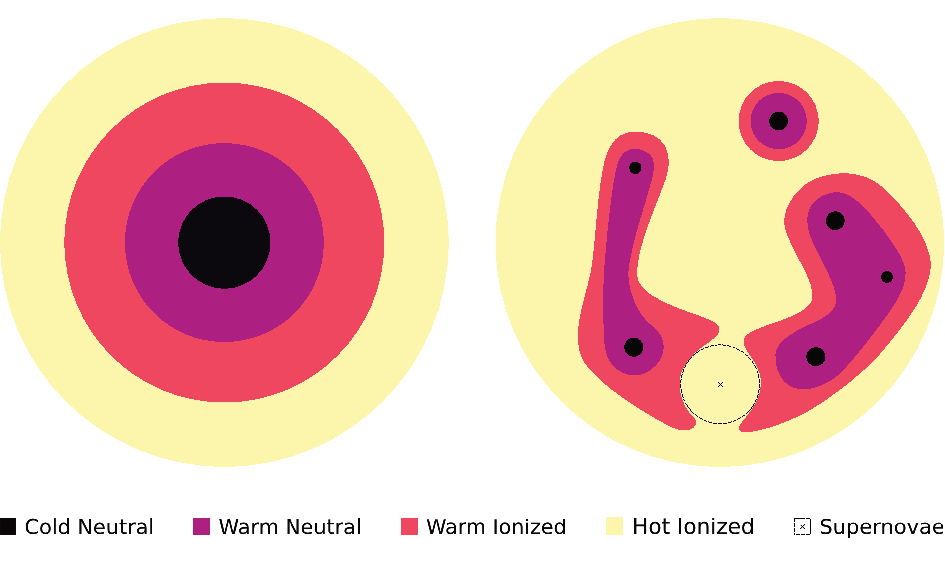
\includegraphics[width=\columnwidth]{structure_v2.pdf}

    \caption{The three-phase structure of the ISM as proposed by \citet{mckee_theory_1977}.
        On the left, the small-scale structure is shown (i.e. one cloud) and on the right the large-scale (with multiple clouds) is shown.
        The large-scale picture aims to show the approximate substructure contained within a single resolution element of a cosmological N-body simulation; this is the region which needs to be `averaged over' to produce a representative subgrid model.
    It should be noted that this figure is for illustration purposes only and does not accurately reflect the relative abundances of the phases; for a more numerical description see \citet{ferriere_interstellar_2001} and the data adapted from it in Table \ref{tab:ism}.}
    \label{fig:struct}
\end{figure}

The study of the substructure of the ISM is important in the development of a subgrid model for within such a model the aim is to take an appropriate `average' over the expected substructure of a given resolution element.
Figure \ref{fig:struct} shows the `standard model' of the structure of the ISM first proposed by \citet{mckee_theory_1977}.
The ISM is made up of three distinct phases, the cold neutral medium, the warm medium, and the hot ionized medium, and these are discussed below.

\subsection{Cold Neutral Phase (H$_2$ gas)}

The cold neutral phase of the ISM is the site of star formation; for a recent overview see \citet{mckee_theory_2007} and associated references.
This phase is dense and cold, and is made up of mainly H$_2$ gas, however it is mainly studied observationally by using a close tracer of H$_2$ gas, CO \citep{ferriere_interstellar_2001}.
The H$_2$ gas forms on the surface of dust grains; even though in these regions the density of gas is high relative to the rest of the ISM, the mean free path between two individual hydrogen atoms still remains high.
The dust grains act as a catalyst as the H atoms are adsorbed onto the surface, which is considerably more likely than a two-body collision of two H atoms \citep{gould_interstellar_1963}.

Within this region, the gas has almost no thermal pressure support ($v_{rms} < 0.5 \kms$), and so is mainly supported by turbulent motions \citep{larson_turbulence_1981, solomon_mass_1987, heyer_universality_2004} with dispersion $\sigma \approx 1 \kms$.
This dispersion is, however, also small, and as such the gas can coalesce and form stars readily in these regions.
Another important property of these regions is that they are shielded from the UV background in the galaxy which is what allows them to reach such cold temperatures; without this shielding the molecular hydrogen would be rapidly dissociated. 

\subsection{Warm Phase (H \textsc{i}, H \textsc{ii})}

The warm phase of the ISM is made up of two sub-components: the warm neutral medium and the warm ionized medium, with both phases having a temperature of $10^4$ K and predominantly being composed of atomic hydrogen (H \textsc{i}) and ionized hydrogen (H \textsc{ii}) respectively.
Above this temperature, the hydrogen can cool radiatively with a high efficiency \citep{gnat_time-dependent_2007}.
The warm neutral medium is shielded by the warm ionized medium (see Figure \ref{fig:struct}); at the surface of the cloud hydrogen is continually ionized and recombining to re-form neutral hydrogen.
This gas is photoionized by the abundant UV photons in the galaxy that are produced by the O and B stars (\citet{lefloch_photoionization_2002} and associated references).

There is a cut-off in star formation at around 3 scale radii from the galactic centre \citep{kennicutt_star_1989, martin_star_2001}, and it is theorised that this is due to a low gas column density at those radii \citep{schaye_star_2004}; in those regions the disk is not dense enough to combat the photoionization and collapse to form stars.
From the theoretical predictions outlined in \citet{schaye_star_2004} and observational data from work such as \citet{bigiel_star_2008} (see Figure \ref{fig:bigielwithmart}), the column density at which star formation is viable appears to be in the range of $2.5 - 10 \msun \pc^{-2}$.

\subsection{Hot Phase (H \textsc{i} +)}

The hot phase of the medium contains ionized hydrogen (H \textsc{i}) and highly ionized metals such as O \textsc{vi} and N \textsc{v} which implies a temperature of $10^{5}$ K and above. The presence of a soft x-ray background at 0.25 keV suggests some regions with a temperature of $10^6 - 10^7$ K \citep{ferriere_interstellar_2001}.

\subsection{Feedback}

Here it becomes clear that there is a feedback loop; cold gas coalesces to form a cloud, the central region of which can form stars that produce UV photons (and hence a region of H \textsc{ii} gas).
Some of the high-mass stars that form in this process will end their lives in a supernova, the shock from which will destroy the cloud and produce a `hot' region with highly ionized metals.
The ISM can then cool through radiative cooling back to $10^4$ K, self-shield and form a molecular cloud if the region remains dense enough.

\subsection{Simulations} 

The only way to see the direct evolution of a molecular cloud and the effects of star formation and supernovae is through high-resolution (typically 1 pc) simulations \citep{martizzi_supernova_2015, girichidis_silcc_2016}.
These simulations give insights into the driving processes for the destruction and formation of molecular clouds and include radiative transfer, stochastic supernovae, the evolution of metals, and many other physical processes that are impossible to include at such high resolutions in a cosmological simulation.
For a `zoom-out' model (such as the one presented here), the small-scale simulations allow for the extraction of macroscopic parameters, which can be used to calibrate a subgrid model for a cosmological or galactic scale simulation.

\begin{table}[hb]
    \centering
    \resizebox{\textwidth}{!}{
        \begin{tabular}{lccc}
            Phase & $T$ [K] & $\rho$ [$n_H \cm^{-3}$]& Observations \\ \hline
            Molecular Gas & $10 - 20$ & $10^2 - 10^6$ & Traced by CO (radio) and IR \\
            Neutral Atomic Gas & $50 - 10000$ & $0.2 - 50$ & Ly$\alpha$ and HI 21 cm radiation \\
            Warm Ionized Gas & $\approx 8000$ & $0.2 - 0.5$ & H$\alpha$ \\
            Hot Ionized Gas & $10^5 - 10^7$ & $10^{-4} - 10^{-2}$ & X-ray and highly ionized metals\\
        \end{tabular}} % end resizebox
    \caption{Overview of the typical densities of the different phases of gas in the ISM, with $T$ the temperature and $\rho$ the gaseous gas density. Data adapted from \citet{ferriere_interstellar_2001}.}
    \label{tab:ism}
\end{table}
